\documentclass[10pt,compress,t,notes=noshow, xcolor=table]{beamer}

\usepackage[]{graphicx}
% graphicx is loaded via lmu-lecture.sty as well
\usepackage[]{color}
% maxwidth is the original width if it is less than linewidth
% otherwise use linewidth (to make sure the graphics do not exceed the margin)
\makeatletter
\def\maxwidth{ %
  \ifdim\Gin@nat@width>\linewidth
    \linewidth
  \else
    \Gin@nat@width
  \fi
}
\makeatother

% ---------------------------------%
% latex-math dependencies, do not remove:
% - mathtools
% - bm
% - siunitx
% - dsfont
% - xspace
% ---------------------------------%

%--------------------------------------------------------%
%       Language, encoding, typography
%--------------------------------------------------------%

\usepackage[english]{babel}
\usepackage[utf8]{inputenc} % Enables inputting UTF-8 symbols
% Standard AMS suite (loaded via lmu-lecture.sty)
\usepackage{amsmath,amsfonts,amssymb}

% Font for double-stroke / blackboard letters for sets of numbers (N, R, ...)
% Distribution name is "doublestroke"
% According to https://mirror.physik.tu-berlin.de/pub/CTAN/fonts/doublestroke/dsdoc.pdf
% the "bbm" package does a similar thing and may be superfluous.
% Required for latex-math
\usepackage{dsfont}

% bbm – "Blackboard-style" cm fonts (https://www.ctan.org/pkg/bbm)
% Used to be in common.tex, loaded directly after this file
% Maybe superfluous given dsfont is loaded
% TODO: Check if really unused?
% \usepackage{bbm}

% bm – Access bold symbols in maths mode - https://ctan.org/pkg/bm
% Required for latex-math, preferred over \boldsymbol
% https://tex.stackexchange.com/questions/3238/bm-package-versus-boldsymbol
\usepackage{bm}

% pifont – Access to PostScript standard Symbol and Dingbats fonts
% Used for \newcommand{\xmark}{\ding{55}, which is never used
% aside from lecture_advml/attic/xx-automl/slides.Rnw
% \usepackage{pifont}

% Quotes (inline and display), provdes \enquote
% https://ctan.org/pkg/csquotes
\usepackage{csquotes}

% Adds arg to enumerate env, technically superseded by enumitem according
% to https://ctan.org/pkg/enumerate
% Replace with https://ctan.org/pkg/enumitem ?
% Even better: enumitem is not really compatible with beamer and breaks all sorts of things
% particularly the enumerate environment. The enumerate package also just isn't required
% from what I can tell so... don't re-add it I guess?
% \usepackage{enumerate}

% Line spacing - provides \singlespacing \doublespacing \onehalfspacing
% https://ctan.org/pkg/setspace
% \usepackage{setspace}

% mathtools – Mathematical tools to use with amsmath
% https://ctan.org/pkg/mathtools?lang=en
% latex-math dependency according to latex-math repo
\usepackage{mathtools}

% Maybe not great to use this https://tex.stackexchange.com/a/197/19093
% Use align instead -- TODO: Global search & replace to check, eqnarray is used a lot
% $ rg -f -u "\begin{eqnarray" -l | grep -v attic | awk -F '/' '{print $1}' | sort | uniq -c
%   13 lecture_advml
%   14 lecture_i2ml
%    2 lecture_iml
%   27 lecture_optimization
%   45 lecture_sl
\usepackage{eqnarray}

% For shaded regions / boxes
% Used sometimes in optim
% https://www.ctan.org/pkg/framed
\usepackage{framed}

%--------------------------------------------------------%
%       Cite button (version 2024-05)
%--------------------------------------------------------%
% Note this requires biber to be in $PATH when running,
% telltale error in log would be e.g. Package biblatex Info: ... file 'authoryear.dbx' not found
% aside from obvious "biber: command not found" or similar.
% Tried moving this to lmu-lecture.sty but had issues I didn't quite understood,
% so it's here for now.

\usepackage{textcase} % for \NoCaseChange
\usepackage{hyperref}

% Only try adding a references file if it exists, otherwise
% this would compile error when references.bib is not found
\IfFileExists{references.bib} {
  \usepackage{usebib}
  \usepackage[backend=biber, style=authoryear]{biblatex}

  \addbibresource{./references.bib}
  \bibinput{references}
}

\newcommand{\citelink}[1]{%
\NoCaseChange{\resizebox{!}{9pt}{\protect\beamergotobutton{\href{\usebibentry{\NoCaseChange{#1}}{url}}{\begin{NoHyper}\cite{#1}\end{NoHyper}}}}}%
}

%--------------------------------------------------------%
%       Displaying code and algorithms
%--------------------------------------------------------%

% Reimplements verbatim environments: https://ctan.org/pkg/verbatim
% verbatim used sed at least once in
% supervised-classification/slides-classification-tasks.tex
% Removed since code should not be put on slides anyway
% \usepackage{verbatim}

% Both used together for algorithm typesetting, see also overleaf: https://www.overleaf.com/learn/latex/Algorithms
% algorithmic env is also used, but part of the bundle:
%   "algpseudocode is part of the algorithmicx bundle, it gives you an improved version of algorithmic besides providing some other features"
% According to https://tex.stackexchange.com/questions/229355/algorithm-algorithmic-algorithmicx-algorithm2e-algpseudocode-confused
\usepackage{algorithm}
\usepackage{algpseudocode}

%--------------------------------------------------------%
%       Tables
%--------------------------------------------------------%

% multi-row table cells: https://www.namsu.de/Extra/pakete/Multirow.html
% Provides \multirow
% Used e.g. in evaluation/slides-evaluation-measures-classification.tex
\usepackage{multirow}

% colortbl: https://ctan.org/pkg/colortbl
% "The package allows rows and columns to be coloured, and even individual cells." well.
% Provides \columncolor and \rowcolor
% \rowcolor is used multiple times, e.g. in knn/slides-knn.tex
\usepackage{colortbl}

% long/multi-page tables: https://texdoc.org/serve/longtable.pdf/0
% Not used in slides
% \usepackage{longtable}

% pretty table env: https://ctan.org/pkg/booktabs
% Is used
% Defines \toprule
\usepackage{booktabs}

%--------------------------------------------------------%
%       Figures: Creating, placing, verbing
%--------------------------------------------------------%

% wrapfig - Wrapping text around figures https://de.overleaf.com/learn/latex/Wrapping_text_around_figures
% Provides wrapfigure environment -used in lecture_optimization
\usepackage{wrapfig}

% Sub figures in figures and tables
% https://ctan.org/pkg/subfig -- supersedes subfigure package
% Provides \subfigure
% \subfigure not used in slides but slides-tuning-practical.pdf errors without this pkg, error due to \captionsetup undefined
\usepackage{subfig}

% Actually it's pronounced PGF https://en.wikibooks.org/wiki/LaTeX/PGF/TikZ
\usepackage{tikz}

% No idea what/why these settings are what they are but I assume they're there on purpose
\usetikzlibrary{shapes,arrows,automata,positioning,calc,chains,trees, shadows}
\tikzset{
  %Define standard arrow tip
  >=stealth',
  %Define style for boxes
  punkt/.style={
    rectangle,
    rounded corners,
    draw=black, very thick,
    text width=6.5em,
    minimum height=2em,
    text centered},
  % Define arrow style
  pil/.style={
    ->,
    thick,
    shorten <=2pt,
    shorten >=2pt,}
}

%--------------------------------------------------------%
%       Beamer setup and custom macros & environments
%--------------------------------------------------------%

% Main sty file for beamer setup (layout, style, lecture page numbering, etc.)
% For long-term maintenance, this may me refactored into a more modular set of .sty files
\usepackage{../../style/lmu-lecture}
% Custom itemize wrappers, itemizeS, itemizeL, etc
\usepackage{../../style/customitemize}
% Custom framei environment, uses custom itemize!
\usepackage{../../style/framei}
% Custom frame2 environment, allows specifying font size for all content
\usepackage{../../style/frame2}
% Column layout macros
\usepackage{../../style/splitV} 

% Used regularly
\let\code=\texttt

% Not sure what/why this does
\setkeys{Gin}{width=0.9\textwidth}

% -- knitr leftovers --
% Used often in conjunction with \definecolor{shadecolor}{rgb}{0.969, 0.969, 0.969}
% Removing definitions requires chaning _many many_ slides, which then need checking to see if output still ok
\definecolor{fgcolor}{rgb}{0.345, 0.345, 0.345}
\definecolor{shadecolor}{rgb}{0.969, 0.969, 0.969}
\newenvironment{knitrout}{}{} % an empty environment to be redefined in TeX

%-------------------------------------------------------------------------------------------------------%
%  Unused stuff that needs to go but is kept here currently juuuust in case it was important after all  %
%-------------------------------------------------------------------------------------------------------%

% \newcommand{\hlnum}[1]{\textcolor[rgb]{0.686,0.059,0.569}{#1}}%
% \newcommand{\hlstr}[1]{\textcolor[rgb]{0.192,0.494,0.8}{#1}}%
% \newcommand{\hlcom}[1]{\textcolor[rgb]{0.678,0.584,0.686}{\textit{#1}}}%
% \newcommand{\hlopt}[1]{\textcolor[rgb]{0,0,0}{#1}}%
% \newcommand{\hlstd}[1]{\textcolor[rgb]{0.345,0.345,0.345}{#1}}%
% \newcommand{\hlkwa}[1]{\textcolor[rgb]{0.161,0.373,0.58}{\textbf{#1}}}%
% \newcommand{\hlkwb}[1]{\textcolor[rgb]{0.69,0.353,0.396}{#1}}%
% \newcommand{\hlkwc}[1]{\textcolor[rgb]{0.333,0.667,0.333}{#1}}%
% \newcommand{\hlkwd}[1]{\textcolor[rgb]{0.737,0.353,0.396}{\textbf{#1}}}%
% \let\hlipl\hlkwb

% \makeatletter
% \newenvironment{kframe}{%
%  \def\at@end@of@kframe{}%
%  \ifinner\ifhmode%
%   \def\at@end@of@kframe{\end{minipage}}%
%   \begin{minipage}{\columnwidth}%
%  \fi\fi%
%  \def\FrameCommand##1{\hskip\@totalleftmargin \hskip-\fboxsep
%  \colorbox{shadecolor}{##1}\hskip-\fboxsep
%      % There is no \\@totalrightmargin, so:
%      \hskip-\linewidth \hskip-\@totalleftmargin \hskip\columnwidth}%
%  \MakeFramed {\advance\hsize-\width
%    \@totalleftmargin\z@ \linewidth\hsize
%    \@setminipage}}%
%  {\par\unskip\endMakeFramed%
%  \at@end@of@kframe}
% \makeatother

% \definecolor{shadecolor}{rgb}{.97, .97, .97}
% \definecolor{messagecolor}{rgb}{0, 0, 0}
% \definecolor{warningcolor}{rgb}{1, 0, 1}
% \definecolor{errorcolor}{rgb}{1, 0, 0}
% \newenvironment{knitrout}{}{} % an empty environment to be redefined in TeX

% \usepackage{alltt}
% \newcommand{\SweaveOpts}[1]{}  % do not interfere with LaTeX
% \newcommand{\SweaveInput}[1]{} % because they are not real TeX commands
% \newcommand{\Sexpr}[1]{}       % will only be parsed by R
% \newcommand{\xmark}{\ding{55}}%

% textpos – Place boxes at arbitrary positions on the LATEX page
% https://ctan.org/pkg/textpos
% Provides \begin{textblock}
% TODO: Check if really unused?
% \usepackage[absolute,overlay]{textpos}

% -----------------------%
% Likely knitr leftovers %
% -----------------------%

% psfrag – Replace strings in encapsulated PostScript figures
% https://www.overleaf.com/latex/examples/psfrag-example/tggxhgzwrzhn
% https://ftp.mpi-inf.mpg.de/pub/tex/mirror/ftp.dante.de/pub/tex/macros/latex/contrib/psfrag/pfgguide.pdf
% Can't tell if this is needed
% TODO: Check if really unused?
% \usepackage{psfrag}

% arydshln – Draw dash-lines in array/tabular
% https://www.ctan.org/pkg/arydshln
% !! "arydshln has to be loaded after array, longtable, colortab and/or colortbl"
% Provides \hdashline and \cdashline
% Not used in slides
% \usepackage{arydshln}

% tabularx – Tabulars with adjustable-width columns
% https://ctan.org/pkg/tabularx
% Provides \begin{tabularx}
% Not used in slides
% \usepackage{tabularx}

% placeins – Control float placement
% https://ctan.org/pkg/placeins
% Defines a \FloatBarrier command
% TODO: Check if really unused?
% \usepackage{placeins}

% Can't find a reason why common.tex is not just part of this file?
% This file is included in slides and exercises

% Rarely used fontstyle for R packages, used only in 
% - forests/slides-forests-benchmark.tex
% - exercises/single-exercises/methods_l_1.Rnw
% - slides/cart/attic/slides_extra_trees.Rnw
\newcommand{\pkg}[1]{{\fontseries{b}\selectfont #1}}

% Spacing helpers, used often (mostly in exercises for \dlz)
\newcommand{\lz}{\vspace{0.5cm}} % vertical space (used often in slides)
\newcommand{\dlz}{\vspace{1cm}}  % double vertical space (used often in exercises, never in slides)
\newcommand{\oneliner}[1] % Oneliner for important statements, used e.g. in iml, algods
{\begin{block}{}\begin{center}\begin{Large}#1\end{Large}\end{center}\end{block}}

% Don't know if this is used or needed, remove?
% textcolor that works in mathmode
% https://tex.stackexchange.com/a/261480
% Used e.g. in forests/slides-forests-bagging.tex
% [...] \textcolor{blue}{\tfrac{1}{M}\sum^M_{m} [...]
% \makeatletter
% \renewcommand*{\@textcolor}[3]{%
%   \protect\leavevmode
%   \begingroup
%     \color#1{#2}#3%
%   \endgroup
% }
% \makeatother


% Defines macros and environments
 
\title{Interpretable Machine Learning}
% \author{LMU}
%\institute{\href{https://compstat-lmu.github.io/lecture_iml/}{compstat-lmu.github.io/lecture\_iml}}
\date{}

\begin{document} 

\titlemeta{
Interpretable Models 1
}{
Inherently Interpretable Models - Motivation
}{
figure/whitebox
}{
%\item What characteristics does an interpretable model have?
\item Why should we use interpretable models?
\item Advantages and disadvantages of interpretable models
}


\begin{frame}{Motivation}
%Achieving interpretability by using interpretable models is the most straightforward approach
%\bigskip
\begin{columns}[T, totalwidth = \textwidth]
    \begin{column}{0.58\textwidth}
    \begin{itemize}
        %\item Obtaining interpretations by using interpretable models is the easiest and least error-prone approach
       \item Achieving interpretability by using interpretable models is the most straightforward approach
         \item Classes of models deemed interpretable:
   \begin{itemize}
  \footnotesize
  \item (Generalized) linear models (LM, GLM)
  \item Generalized additive models (GAM)
  \item Decision trees
  \item Rule-based learning
  \item Model-based / component-wise boosting
  \item ...
\end{itemize}
    \end{itemize}
    

    \end{column}
    \begin{column}{0.42\textwidth}  %%<--- here
    \centering
  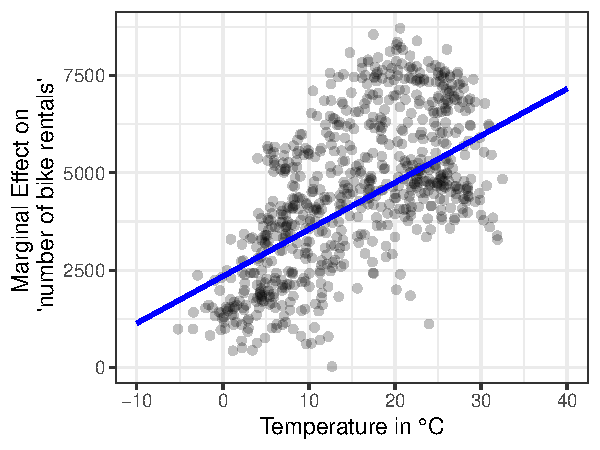
\includegraphics[width = 0.8\textwidth]{figure/main_effect_lm_temp.pdf}
  \begin{center}
    $\leadsto$ LM provides straightforward interpretation
  \end{center}

    \end{column}
\end{columns}

\begin{itemize}
 \item Often there is a trade-off between interpretability and model performance 
        %(but not always)
\end{itemize}
\centering
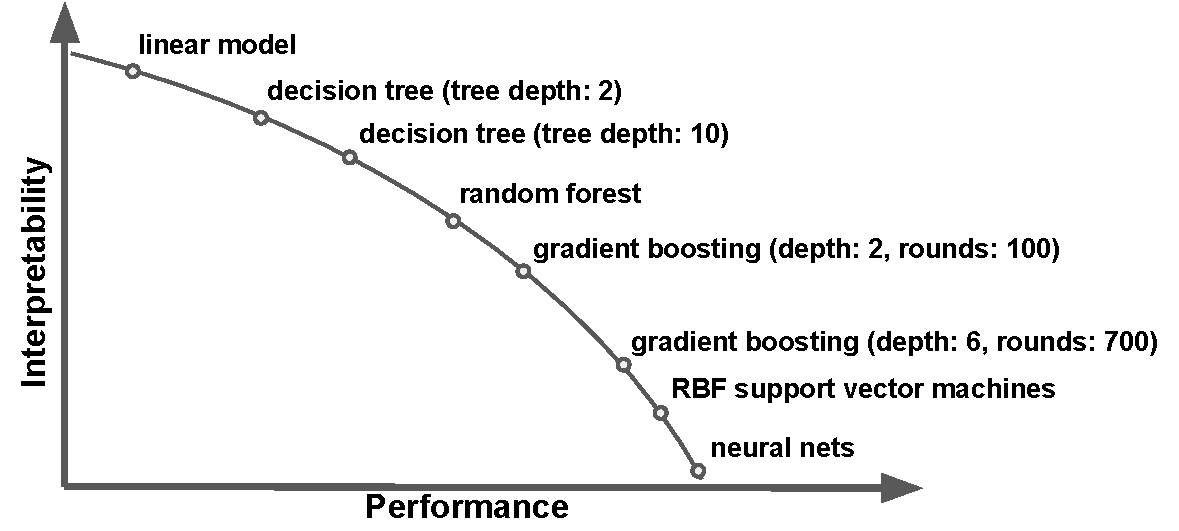
\includegraphics[width=0.55\textwidth]{figure/performance_vs_interpretability.pdf}
    % Quelle: https://docs.google.com/presentation/d/12ZPrTjBKEUT-7drdyUJCQGK0oHVDtYIVd2_6byE62f0/edit?usp=sharing
\end{frame}

\begin{frame}{Advantages}
\begin{columns}[T, totalwidth=\textwidth]
\begin{column}{0.8\textwidth}
    \begin{itemize}[<+->]
    \itemsep1em
        \item Interpretable models are transparent by design, making many model-agnostic explanation methods unnecessary\\
        %For inherently interpretable models some additional model-agnostic interpretation methods not required \\
        $\leadsto$ Eliminates an extra source of estimation error
        \item They often have few hyperparameters and are structurally simple (e.g., linear, additive, sparse, monotonic)\\
        $\leadsto$ Easy to train, fast to tune, straightforward to explain
        % \item Interpretable models often simple \\
        % $\leadsto$ training time is fairly small
        % \item Some interpretable models estimate monotonic effects \\
        % %the monotonicity constraint \\
        % $\leadsto$ Simple to explain as larger feature values always lead to higher (or smaller) outcomes (e.g., GLMs)
        \item Many people are familiar with simple interpretable models \\
        $\leadsto$ Increases trust, facilitates communication of results
        %\item Implementations are available in many programming languages \\
        %$\leadsto$ Simple models are easier to deploy in practice or implement from scratch
    \end{itemize}
\end{column}
\begin{column}{0.2\textwidth}
    \begin{center}
        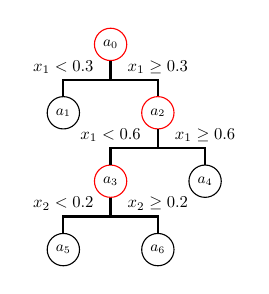
\begin{tikzpicture}[scale=0.6, transform shape]
        \usetikzlibrary{arrows}
            \usetikzlibrary{shapes}
            \tikzset{treenode/.style={draw, circle, font=\small}}
            \tikzset{line/.style={draw, thick}}
            \node [treenode, draw=red] (a0) {$a_0$};
            \node [treenode, below=0.75cm of a0, xshift=-1cm]  (a1) {$a_1$};
            \node [treenode, draw=red, below=0.75cm of a0, xshift=1cm]  (a2) {$a_2$};
     
            \node [treenode, draw=red, below=0.75cm of a2, xshift=-1cm] (a3) {$a_3$};
            \node [treenode, below=0.75cm of a2, xshift=1cm]  (a4) {$a_4$};
     
            \node [treenode, below=0.75cm of a3, xshift=-1cm] (a5) {$a_5$};
            \node [treenode, below=0.75cm of a3, xshift=1cm]  (a6) {$a_6$};
     
            \path [line] (a0.south) -- + (0,-0.4cm) -| (a1.north) node [midway, above] {$x_1<0.3$};
            \path [line] (a0.south) -- +(0,-0.4cm) -|  (a2.north) node [midway, above] {$x_1\geq0.3$};
     
            \path [line] (a2.south) -- + (0,-0.4cm) -| (a3.north) node [midway, above] {$x_1<0.6$};;
            \path [line] (a2.south) -- +(0,-0.4cm) -|  (a4.north) node [midway, above] {$x_1\geq0.6$};
     
          
            \path [line] (a3.south) -- + (0,-0.4cm) -| (a5.north) node [midway, above] {$x_2<0.2$};;
            \path [line] (a3.south) -- +(0,-0.4cm) -|  (a6.north) node [midway, above] {$x_2\geq0.2$};
     
        \end{tikzpicture}
        
        \vspace{0.5cm}
        
        \includegraphics<2->[width = \textwidth]{figure/main_effect_lm_temp.pdf}
    \end{center}
\end{column}
\end{columns}
\end{frame}

\begin{frame}{Disadvantages \& Limitations}
\begin{columns}[totalwidth=\textwidth]
\begin{column}{0.8\textwidth}
    \begin{itemize}%[<+->]
    \itemsep1em
        \item<1-> Often require assumptions about data / model structure \\%Often certain assumptions about data / model structure required\\
        $\leadsto$ If assumptions are wrong, models may perform bad 
        %\item In high-dimensional settings, it may not be feasible to find and define all feature relationships
        %\item If the wrong assumptions are made, interpretable models may have a bad predictive performance
        %\pause
        \item<2-> Interpretable models may also be hard to interpret, e.g.:
    \begin{itemize}
        \item LM with lots of features and interactions 
        \item Decision trees with huge tree depth
    \end{itemize}
    \end{itemize}
\end{column}
\begin{column}{0.2\textwidth}
    \begin{center}
        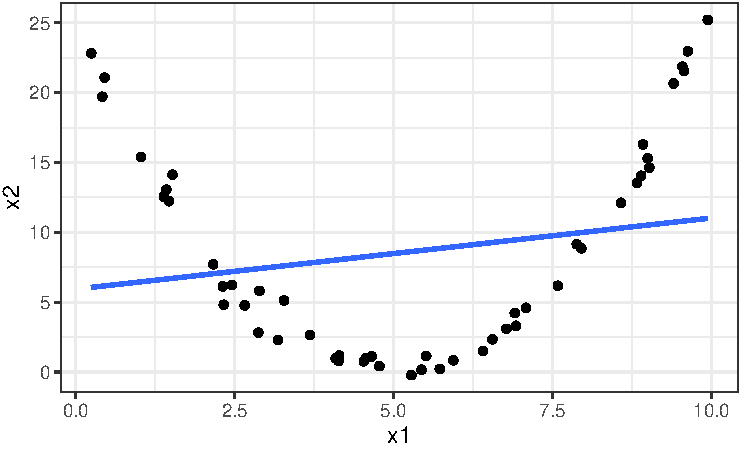
\includegraphics[width = \textwidth]{figure/lm_bad_fit.pdf} 
    \end{center}
\end{column}
\end{columns}
\quad \\

\begin{itemize}
\itemsep1em
        \item<3-> 
        %No automatic modeling of complex relationships due to limited model flexibility
        Often do not automatically model complex relationships due to limited flexibility % didn't find a way to fig the hanging word
        \\
        e.g., high-order main or interaction effects need to be specified manually in an LM

        %\pause
     \item<4-> Inherently interpretable models do not address all explanation needs\\
$\leadsto$ Complementary model-agnostic methods (e.g., counterfactuals) remain valuable for specific tasks
     % Inherently interpretable models do not provide all types of explanations
     % %% one might be interested
     % \\
     % $\leadsto$ Methods providing other types of explanations still useful  (e.g., counterfactual explanations)
     %Methods providing other types of explanations still useful  (e.g., counterfactual explanations)
     %Still requires application of model-agnostic interpretation techniques if certain types of explanations are of interest (e.g., counterfactual explanations)
\end{itemize}
\end{frame}

\begin{frame}{Further Comments}

    \begin{itemize}
    %\itemsep1em
        \item<1-> Some researchers advocate for inherently interpretable models instead of explaining black boxes after training \furtherreading{RUDIN2019}
        \begin{itemize}
        \item Built-in interpretation\\
        $\leadsto$ fewer risks from misleading post-hoc explanations
        
            %\item \ldots instead of explaining uninterpretable models post-hoc
            % \item Can sometimes work out by spending enough time and energy on data pre-processing or manual feature engineering
        \item  Good performance possible with effort on preprocessing and/or feature engineering
        \item But interpretability depends on meaning of created features\\
        $\leadsto$ E.g., PCA keeps models linear, but yields hard-to-interpret components
                %, or data cleaning
        \end{itemize}
        %\pause
        %\footnote[frame]{Rudin, C. Stop explaining black box machine learning models for high stakes decisions and use interpretable models instead. Nat Mach Intell 1, 206–215 (2019).}
        % {https://www.nature.com/articles/s42256-019-0048-x}
       %\item Interpretable models also have the potential for a high predictive performance, but require more knowledge and time spent on data preprocessing
       % \item<2->[$\leadsto$] Drawback: Hard to achieve for data for which end-to-end learning is crucial\\ 
       % $\leadsto$ e.g., hard to extract good features for image / text data\\ 
       % $\leadsto$ information loss can lead to bad performance
      \item<2-> Limitation: Less suited for complex data complex data requiring end-to-end learning
\begin{itemize}
    \item Applies to image, text, or sensor data where features must be learned from raw input
    \item Manual extraction of interpretable features is difficult \\$\Rightarrow$ Information loss and lower performance
\end{itemize}
       %(e.g., for image / text data extraction of good features is hard $\leadsto$ information loss = bad performance)
       %(e.g., image and text data would require good feature extraction steps $\leadsto$ information loss)
        %\pause
        %\item One can assume a trade-off between interpretability and model performance which generally (but not always) holds
        %\item<3-> Often there is a trade-off between interpretability and model performance 
        %(but not always)
    \end{itemize}
    
    %\smallskip
    
    %\only<3>{\centering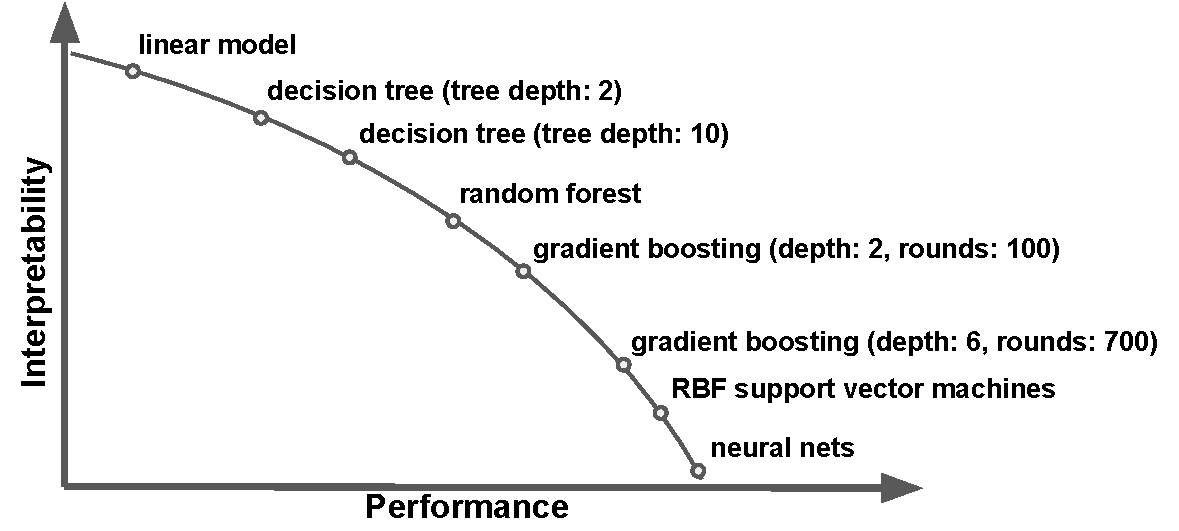
\includegraphics[width=0.65\textwidth]{figure/performance_vs_interpretability.pdf}}
    % Quelle: https://docs.google.com/presentation/d/12ZPrTjBKEUT-7drdyUJCQGK0oHVDtYIVd2_6byE62f0/edit?usp=sharing

\end{frame}


\begin{frame}{Recommendation}
    % \begin{itemize}
    %     \item Start with most simple model that makes sense for application at hand
    %     \item Gradually increase complexity if performance is insufficient\\
    %     $\leadsto$ will usually lower interpretability and require additional interpretation methods
    %     \item Choose the most simple, sufficient model (Occam's razor)
    % \end{itemize} 
\begin{itemize}
    \item Begin with the simplest model appropriate for the task
    \item Increase complexity only if necessary to meet performance requirements\\
    $\leadsto$ Typically reduces interpretability and requires model-agnostic explanations
    \item Choose the simplest model with sufficient accuracy 
    $\leadsto$ Occam’s razor
\end{itemize}
    \bigskip

% \begin{columns}[T, totalwidth=\textwidth]
% \begin{column}{0.5\textwidth}
% \centering \textbf{Bike Data}
%     \begin{table}[ht]
%         \centering
%         \begin{tabular}{lrr}
%             \hline
%             Model & RMSE & $R^2$ \\ 
%             \hline
%             LM & 142.39 & 0.38 \\ 
%             Tree & 98.71 & 0.70 \\ 
%             Random Forest & 57.07 & 0.90 \\ 
%             Boosting & 197.42 & -0.18 \\  
%             \hline
%         \end{tabular}
%     \end{table}
% \end{column}
% \begin{column}{0.5\textwidth}
% \centering \textbf{Boston Housing Data}
%     \begin{table}[ht]
%         \centering
%         \begin{tabular}{lrr}
%             \hline
%             Model & RMSE & $R^2$ \\ 
%             \hline
%             LM & 0.43 & 1.00 \\ 
%             Tree & 1.81 & 0.96 \\ 
%             Random Forest & 1.77 & 0.96 \\ 
%             Boosting & 16.89 & -2.43 \\
%             \hline
%         \end{tabular}
%     \end{table}
% \end{column}
% \end{columns}
% code for tables in rsrc/tab_ml_comparison.R

\centering \textbf{Bike Data, 4-fold CV}
\begin{table}[ht]
\centering
\begin{tabular}{lrr}
  \hline
Model & RMSE & $R^2$ \\ 
  \hline
  LM & 800.15 & 0.83 \\ 
  Tree & 981.83 & 0.74 \\ 
  Random Forest & 653.25 & 0.88 \\ 
  Boosting (tuned) & 638.42 & 0.89 \\ 
   \hline
\end{tabular}
\end{table}
\end{frame}



\endlecture
\end{document}
